
%(BEGIN_QUESTION)
% Copyright 2006, Tony R. Kuphaldt, released under the Creative Commons Attribution License (v 1.0)
% This means you may do almost anything with this work of mine, so long as you give me proper credit

A mixing vessel in a wastewater treatment plant receives water at varying levels of pH, and the control system's task is to maintain the outgoing water pH around 7 (neutral) by adding acid or caustic as needed.  If the incoming water is too acidic (pH below 7), the system should add more caustic; if the incoming water is too alkaline (pH above 7), the system should add more acid:

$$\includegraphics[width=15.5cm]{i01395x01.eps}$$

If the incoming pH is below 7 (acidic), then the control system needs to open the caustic valve to increase the outflow pH.  If the incoming pH is above 7 (caustic), then the control system needs to open the acid valve to decrease the outflow pH.  It would be wasteful, however, to add both acid {\it and} caustic to the mixing vessel at the same time, as they would tend to nullify each other.

How is it possible to operate the acid/caustic valves in such a manner from a single controller?  Sketch a solution into the above P\&ID to show how you would accomplish this.

\vskip 20pt \vbox{\hrule \hbox{\strut \vrule{} {\bf Suggestions for Socratic discussion} \vrule} \hrule}

\begin{itemize}
\item{} A good problem-solving technique to apply in cases where we need to determine the direction of a change is to consider {\it limiting cases}.  Instead of asking ourselves what would happen if the pH changes slightly, we ask ourselves what would happen if the pH changes {\it dramatically}.  Explain how this problem-solving technique applies to this particular system where we must determine necessary controller action and final control element sequencing.
\item{} What do the arrow symbols on the valve stems represent?
\item{} Identify the consequence of losing instrument air to the control valves -- what will happen to the effluent pH?
\item{} Identify the consequence of a failed-open 4-20 mA cable in your proposed solution -- what will happen to the effluent pH?
\item{} Identify alternative split-range sequencing configurations (other than the one you proposed in your answer).
\end{itemize}

\underbar{file i01395}
%(END_QUESTION)





%(BEGIN_ANSWER)

This is one way to connect the valves together as a split-ranged pair:

$$\includegraphics[width=15.5cm]{i01395x02.eps}$$

%(END_ANSWER)





%(BEGIN_NOTES)

What we need is this form of split-ranging, assuming a {\it reverse-acting} controller:

$$\includegraphics[width=15.5cm]{i01395x03.eps}$$

The two I/P transducers (``AY'' devices) will both have output ranges of 3-15 PSI, but one will have an input range of 4-12 mA while the other has an input range of 12-20 mA.

\vskip 10pt

Another possibility is to use a single I/P transducer and amplify its output using two pneumatic multiplying relays: one with an input range of 3-9 PSI and an output range of 3-15 PSI, and the other with an input range of 9-15 PSI and an output range of 3-15 PSI.  This technique of using two pneumatic amplifying relays makes more sense, though, when the controller output is pneumatic.  If the controller in question is electronic, it makes more sense to use two I/P transducers rather than one I/P transducer and two amplifying relays.

Incidentally, the generic measured-variable letter for any analytical (chemistry-sensing) instrument is ``A,'' and since pH is a form of chemical measurement, ``AT'' is appropriate to describe a pH transmitter.  Note the letters ``pH'' to the upper-right of the transmitter bubble symbol, placed there to further specify that transmitter's function.  However, it is also proper to use the letters ``pH'' to label instruments in a pH loop.  So, we could have labeled the analyzer (transmitter) ``pHT'' and the indicating controller ``pHIC'' instead of ``AT'' and ``AIC.''  In like manner, the two I/P transducers could have each been labeled ``pHY'' instead of ``AY.''

%INDEX% Final Control Elements, valve: split ranging
%INDEX% Process: water pH neutralization (generic)

%(END_NOTES)


